\documentclass[12pt]{article}

\usepackage[english]{babel}
\usepackage[iso,english]{isodate}
\usepackage[table,svgnames]{xcolor}
\usepackage{cmbright}
\usepackage{url}
\usepackage[utf8x]{inputenc}
\usepackage[T1]{fontenc}
\usepackage{longtable}
\usepackage{amsmath}
\usepackage{graphicx}
\usepackage{parskip}
\usepackage{fancyhdr}
\usepackage{vmargin}
\usepackage{hyperref}
\usepackage{pgfgantt}
\usepackage{pgf-umlcd}
\usepackage{xparse}
\usepackage{float}
\usepackage{tikz}
\usepackage{tabularx}
\usepackage{titling}
\usepackage[nogroupskip,toc,acronym]{glossaries}
\usepackage{fancyhdr}
\usepackage[authoryear]{natbib}
\usepackage{enumitem}
\usepackage{rotating}
%\bibliographystyle{fontysIEEtranN}

\pagestyle{fancy}
\fancyhf{}
\lhead{
\includegraphics[width=0.2\linewidth]{TreewatchLogo.pdf}}
\rhead{Personal dossier Ron Gebauer}
\rfoot{Page \thepage}

% alternate row colors for all tables
\definecolor{lightGrey}{rgb}{0.95,0.95,0.95}

\let\oldtable\table
\let\endoldtable\endtable
\renewenvironment{table}{\rowcolors{2}{lightGrey}{}\oldtable}{\endoldtable}

\let\oldtabular\tabular
\let\endoldtabular\endtabular
\renewenvironment{tabular}{\rowcolors{2}{lightGrey}{}\oldtabular}{\endoldtabular}

\let\oldtabularx\tabularx
\let\endoldtabularx\endtabularx
\renewenvironment{tabularx}{\rowcolors{2}{lightGrey}{}\oldtabularx}{\endoldtabularx}

\let\oldlongtable\longtable
\let\endoldlongtable\endlongtable
\renewenvironment{longtable}{\rowcolors{2}{lightGrey}{}\oldlongtable} {\endoldlongtable}

\graphicspath{{../../img/}{../img/personaldossiers/ron/}}

\renewcommand{\arraystretch}{1.5}

\DeclareDocumentCommand{\newdualentry}{ O{} O{} m m m m } {
  \newglossaryentry{gls-#3}{name={#5},text={#5\glsadd{#3}},
    description={#6},#1
  }
  \makeglossaries
  \newacronym[see={[Glossary:]{gls-#3}},#2]{#3}{#4}{#5\glsadd{gls-#3}}
}


\newlist{SMART}{description}{2}
\setlist[SMART]{leftmargin=6.5em,style=nextline}

\newlist{STARR}{description}{2}
\setlist[STARR]{leftmargin=5.5em,style=nextline}


%\loadglsentries{../glossary.tex}

\setmarginsrb{3 cm}{2.5 cm}{3 cm}{2.5 cm}{1 cm}{1.5 cm}{1 cm}{1.5 cm}

%\makeglossaries
\begin{document}

%%%%%%%%%%%%%%%%%%%%%%%%%%%%%%%%%%%%%%%%%%%%%%%%%%%%%%%%%%%%%%%%%%%%%%%%%%%%%%%%%%%%%%%%% Preface of the report

    \pagenumbering{Roman} % Roman numerals for page counter


    % Title Page
    \begin{titlingpage}
        \begin{center}
            \begin{minipage}{\linewidth}
            \centering
            %University logo
            
\includegraphics[width=0.3\linewidth]{FontysLogo.pdf}
            \par
            \vspace{3cm}
            %Thesis title
            {\uppercase
                {\Large Personal dossier\\ Ron Gebauer \\ 2015 Sofa GTL \\ TreeWatch Project
            \par
            \vspace{3cm}}}
            
\includegraphics[width=0.5\linewidth]{TreewatchLogo.pdf}
            \par
            \vspace{2cm}
            %Author's name
            {Ron Gebauer\\
	         \par}
            \vspace{2cm}

            %Date
            \today
            \end{minipage}
        \end{center}
    \end{titlingpage}
    \clearpage

    \setmarginsrb{3 cm}{2.5 cm}{3 cm}{2.5 cm}{1.5 cm}{1.5 cm}{1 cm}{1.5 cm}
    \section*{Document information}
\addcontentsline{toc}{section}{Document information}
\renewenvironment{tabular}{\oldtabular}{\endoldtabular}
	\begin{tabular}{ll}
		\textbf{Document name:} & Personal Dossier Ron Gebauer\\
		\textbf{Document owner:} & Ron Gebauer \\
		\textbf{Company/Organisation:} & Fleuren Baarlo \\
		\textbf{Contact person:} & Ron Gebauer \\
		\textbf{Date:} & \today \\
		\textbf{Place:} & Fontys University of Applied Science Venlo \\
		\textbf{Author:} & \parbox[t]{5cm}{
				Ron Gebauer\\
				r.gebauer@student.fontys.nl\\
				2153294
			}
	\end{tabular}
\renewenvironment{tabular}{\rowcolors{2}{lightGrey}{}\oldtabular}{\endoldtabular}

    %\printglossary[type=\acronymtype]
    %\printglossary
    \pagebreak

    %\listoffigures
    %\addcontentsline{toc}{section}{\listfigurename}
    %\listoftables
    %\addcontentsline{toc}{section}{\listtablename}
    %\pagebreak

    \tableofcontents
    \clearpage

%%%%%%%%%%%%%%%%%%%%%%%%%%%%%%%%%%%%%%%%%%%%%%%%%%%%%%%%%%%%%%%%%%%%%%%%%%%%%%%%%%%%%%%%% Main Part of the Report

    \pagenumbering{arabic}
   
	\section{Improve Programming Skills}
	\subsection{Reason to Choose}
		The topic of the Software Factory is completely new, which is the reason why I would like to improve my development skills in that kind of topics.

	\subsection{S.M.A.R.T.}
		\begin{SMART}
			\item[Specific] As my personal learning goal I want to improve my knowledge of the program language used in the project. The programming language used is not yet clear.
			\item[Measurable] This is measured by the result of the division of compiler errors by lines of code.
			\item[Attainable] Information about the programming language used may be found on the Internet but also in various books or ebooks.
			\item[Relevant] There are many programming languages but they can not all mastered. To have many options after graduation, you should have a lot of them already programmed.
			\item[Time-limited] The semester ends in January 2016 which is why I will have reached my goal by the end of January.
		\end{SMART}

	\subsection{S.T.A.R.R.}
		\begin{STARR}
			\item[Situation] We were using Xamarin Studio together with a student license to develop our product. Inside Xamarin the solution was written in C\# and separated into different projects for every platform. One project was for cross-platform development, which was also my main playground inside our project.
			\item[Task] I wanted to mainly improve my programming skills inside a cross-platform application.
			\item[Action] Inside the project I worked mainly inside the cross-platform project but also the iOS and the Android project got some attention. At first I built the complete main view structure and implemented it. For that the graph at the end of this sub section will show how does it work.

				Furthermore I invent together with Martijn Bonajo, a group member of my group, the MVVM pattern inside our cross-platform project.
				
			\item[Result] The results can be found in our group dossier in chapter 15 sections 1 to 25 and section 44.
			
				The compiler errors while I was programming was not so much I thought it would be. But unfortunately I had one compiler error every 100 lines of code.
			\item[Reflection] More or less I learned a lot about the MVVM Pattern used in Xamarin Studio. I think the next time I need to create an application front end I will definitely work more in that way.
		\end{STARR}
		
		\hspace*{4cm}
		\begin{turn}{90}
			\usetikzlibrary{trees}
			\tikzstyle{every node}=[draw=black,thick,anchor=west]
			\begin{tikzpicture}[%
				grow via three points={one child at (0.5,-0.7) and
				two children at (0.5,-0.7) and (0.5,-1.4)},
				edge from parent path={(\tikzparentnode.south) |- (\tikzchildnode.west)}]
				\node {TreeWatch Application}
					child { node {Map}
				    	child { node {Map Menu}}
				    	child { node {Field Informations}
					    	child { node {Variety Informations}
				    			child { node {Blocks Informations}
							    	child { node {Block Informations}}
						    	}
				    		}
				    	}
					}
					child [missing] { node {Note}}
					child [missing] { node {Note}}
					child { node {Note}}
					child { node {ToDo}}
					child { node {History}}
					child { node {Settings}
				    	child { node {Map Type Selection}}
				    };
			\end{tikzpicture}
		\end{turn}
	
	\section{Improve Skills of a Scrum Master}
	\subsection{Reason to Choose}
		In the project during the 7th semester, which is the Software Factory, I chose the position of a Scrum Master. To successfully fill in this position and being able to support my group I wanted to improve my knowledge of this position during that semester.
		My decision was made for the following learning goal because of this reason.

	\subsection{S.M.A.R.T.}
	\begin{SMART}
	    \item[Specific] As the Scrum Master in our project, I want to improve my skills for this task.
	    \item[Measurable] This competence can be measured using a small questionnaire, because my team members can tell the best if I have made myself well.
	    \item[Attainable] To improve my skills in this area, I can find lots of information on the Internet but also benefit from the experience of my group.
	    \item[Relevant] Scrum is a methodology in many software projects of small and large companies.
	    \item[Time-limited] The semester ends in January 2016 which is why I will have reached my goal by the end of January.
	\end{SMART}
	
	\subsection{S.T.A.R.R.}
	\begin{STARR}
	    \item[Situation] 
	    \item[Task] 
	    \item[Action] 
	    \item[Result] 
	    \item[Reflection] 
	\end{STARR}

	\section{Improve a Proactive}
	\subsection{Reason to Choose}
		

	\subsection{SMART}
		\begin{SMART}
		    \item[Specific] A proactive for me is to be present and on time. That's one of my biggest weaknesses.
		    \item[Measurable] This can be measured by a statistical comparison of the times when I was on time and unpunctual. In addition, you can compare my arrival and absent-ness percentage together.
		    \item[Attainable] In the present time appointments, work schedules and events are an integral part and therefore time management is a very important issue.
		    \item[Relevant] This is a very relevant issue, as it could cost me my job if I am too often absent or late.
		    \item[Time-limited] The semester ends in January 2016 which is why I will have reached my goal by the end of January.
		\end{SMART}
	
	\subsection{STAR}
		\begin{STAR}
		    \item[Situation] 
		    \item[Task] 
		    \item[Action] 
		    \item[Result] 
		\end{STAR}
		
		\begin{figure}[htbp]
			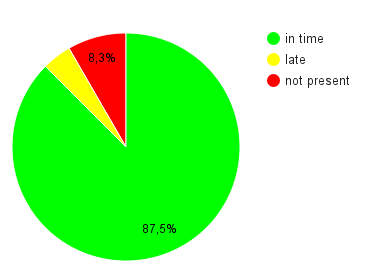
\includegraphics[width=\textwidth]{../img/inTimeDiagramm}
		\end{figure}

%\clearpage

%\bibliography{biblist}

\end{document}
